% Options for packages loaded elsewhere
\PassOptionsToPackage{unicode}{hyperref}
\PassOptionsToPackage{hyphens}{url}
%
\documentclass[
  man]{apa6}
\usepackage{amsmath,amssymb}
\usepackage{lmodern}
\usepackage{iftex}
\ifPDFTeX
  \usepackage[T1]{fontenc}
  \usepackage[utf8]{inputenc}
  \usepackage{textcomp} % provide euro and other symbols
\else % if luatex or xetex
  \usepackage{unicode-math}
  \defaultfontfeatures{Scale=MatchLowercase}
  \defaultfontfeatures[\rmfamily]{Ligatures=TeX,Scale=1}
\fi
% Use upquote if available, for straight quotes in verbatim environments
\IfFileExists{upquote.sty}{\usepackage{upquote}}{}
\IfFileExists{microtype.sty}{% use microtype if available
  \usepackage[]{microtype}
  \UseMicrotypeSet[protrusion]{basicmath} % disable protrusion for tt fonts
}{}
\makeatletter
\@ifundefined{KOMAClassName}{% if non-KOMA class
  \IfFileExists{parskip.sty}{%
    \usepackage{parskip}
  }{% else
    \setlength{\parindent}{0pt}
    \setlength{\parskip}{6pt plus 2pt minus 1pt}}
}{% if KOMA class
  \KOMAoptions{parskip=half}}
\makeatother
\usepackage{xcolor}
\usepackage{graphicx}
\makeatletter
\def\maxwidth{\ifdim\Gin@nat@width>\linewidth\linewidth\else\Gin@nat@width\fi}
\def\maxheight{\ifdim\Gin@nat@height>\textheight\textheight\else\Gin@nat@height\fi}
\makeatother
% Scale images if necessary, so that they will not overflow the page
% margins by default, and it is still possible to overwrite the defaults
% using explicit options in \includegraphics[width, height, ...]{}
\setkeys{Gin}{width=\maxwidth,height=\maxheight,keepaspectratio}
% Set default figure placement to htbp
\makeatletter
\def\fps@figure{htbp}
\makeatother
\setlength{\emergencystretch}{3em} % prevent overfull lines
\providecommand{\tightlist}{%
  \setlength{\itemsep}{0pt}\setlength{\parskip}{0pt}}
\setcounter{secnumdepth}{-\maxdimen} % remove section numbering
% Make \paragraph and \subparagraph free-standing
\ifx\paragraph\undefined\else
  \let\oldparagraph\paragraph
  \renewcommand{\paragraph}[1]{\oldparagraph{#1}\mbox{}}
\fi
\ifx\subparagraph\undefined\else
  \let\oldsubparagraph\subparagraph
  \renewcommand{\subparagraph}[1]{\oldsubparagraph{#1}\mbox{}}
\fi
\newlength{\cslhangindent}
\setlength{\cslhangindent}{1.5em}
\newlength{\csllabelwidth}
\setlength{\csllabelwidth}{3em}
\newlength{\cslentryspacingunit} % times entry-spacing
\setlength{\cslentryspacingunit}{\parskip}
\newenvironment{CSLReferences}[2] % #1 hanging-ident, #2 entry spacing
 {% don't indent paragraphs
  \setlength{\parindent}{0pt}
  % turn on hanging indent if param 1 is 1
  \ifodd #1
  \let\oldpar\par
  \def\par{\hangindent=\cslhangindent\oldpar}
  \fi
  % set entry spacing
  \setlength{\parskip}{#2\cslentryspacingunit}
 }%
 {}
\usepackage{calc}
\newcommand{\CSLBlock}[1]{#1\hfill\break}
\newcommand{\CSLLeftMargin}[1]{\parbox[t]{\csllabelwidth}{#1}}
\newcommand{\CSLRightInline}[1]{\parbox[t]{\linewidth - \csllabelwidth}{#1}\break}
\newcommand{\CSLIndent}[1]{\hspace{\cslhangindent}#1}
\ifLuaTeX
\usepackage[bidi=basic]{babel}
\else
\usepackage[bidi=default]{babel}
\fi
\babelprovide[main,import]{english}
% get rid of language-specific shorthands (see #6817):
\let\LanguageShortHands\languageshorthands
\def\languageshorthands#1{}
% Manuscript styling
\usepackage{upgreek}
\captionsetup{font=singlespacing,justification=justified}

% Table formatting
\usepackage{longtable}
\usepackage{lscape}
% \usepackage[counterclockwise]{rotating}   % Landscape page setup for large tables
\usepackage{multirow}		% Table styling
\usepackage{tabularx}		% Control Column width
\usepackage[flushleft]{threeparttable}	% Allows for three part tables with a specified notes section
\usepackage{threeparttablex}            % Lets threeparttable work with longtable

% Create new environments so endfloat can handle them
% \newenvironment{ltable}
%   {\begin{landscape}\begin{center}\begin{threeparttable}}
%   {\end{threeparttable}\end{center}\end{landscape}}
\newenvironment{lltable}{\begin{landscape}\begin{center}\begin{ThreePartTable}}{\end{ThreePartTable}\end{center}\end{landscape}}

% Enables adjusting longtable caption width to table width
% Solution found at http://golatex.de/longtable-mit-caption-so-breit-wie-die-tabelle-t15767.html
\makeatletter
\newcommand\LastLTentrywidth{1em}
\newlength\longtablewidth
\setlength{\longtablewidth}{1in}
\newcommand{\getlongtablewidth}{\begingroup \ifcsname LT@\roman{LT@tables}\endcsname \global\longtablewidth=0pt \renewcommand{\LT@entry}[2]{\global\advance\longtablewidth by ##2\relax\gdef\LastLTentrywidth{##2}}\@nameuse{LT@\roman{LT@tables}} \fi \endgroup}

% \setlength{\parindent}{0.5in}
% \setlength{\parskip}{0pt plus 0pt minus 0pt}

% \usepackage{etoolbox}
\makeatletter
\patchcmd{\HyOrg@maketitle}
  {\section{\normalfont\normalsize\abstractname}}
  {\section*{\normalfont\normalsize\abstractname}}
  {}{\typeout{Failed to patch abstract.}}
\patchcmd{\HyOrg@maketitle}
  {\section{\protect\normalfont{\@title}}}
  {\section*{\protect\normalfont{\@title}}}
  {}{\typeout{Failed to patch title.}}
\makeatother
\shorttitle{Language Input to Blind Infants/Toddlers}
\keywords{keywords\newline\indent Word count: X}
\DeclareDelayedFloatFlavor{ThreePartTable}{table}
\DeclareDelayedFloatFlavor{lltable}{table}
\DeclareDelayedFloatFlavor*{longtable}{table}
\makeatletter
\renewcommand{\efloat@iwrite}[1]{\immediate\expandafter\protected@write\csname efloat@post#1\endcsname{}}
\makeatother
\usepackage{lineno}

\linenumbers
\usepackage{csquotes}
\ifLuaTeX
  \usepackage{selnolig}  % disable illegal ligatures
\fi
\IfFileExists{bookmark.sty}{\usepackage{bookmark}}{\usepackage{hyperref}}
\IfFileExists{xurl.sty}{\usepackage{xurl}}{} % add URL line breaks if available
\urlstyle{same} % disable monospaced font for URLs
\hypersetup{
  pdftitle={Language Input to Blind Infants/Toddlers},
  pdfauthor={Erin Campbell1, Lillianna Righter1, \& Elika Bergelson1},
  pdflang={en-EN},
  pdfkeywords={keywords},
  hidelinks,
  pdfcreator={LaTeX via pandoc}}

\title{Language Input to Blind Infants/Toddlers}
\author{Erin Campbell\textsuperscript{1}, Lillianna Righter\textsuperscript{1}, \& Elika Bergelson\textsuperscript{1}}
\date{}


\note{

\textbf{Conflicts of Interest}: The authors have no conflicts of interest to report.
\textbf{Funding}: This work was supported by the National Science Foundation CAREER grant (BCS-1844710) to EB and Graduate Research Fellowship (2019274952) to EC.

}

\affiliation{\vspace{0.5cm}\textsuperscript{1} Department of Psychology \& Neuroscience, Duke University, Durham, NC}

\begin{document}
\maketitle

\hypertarget{introduction}{%
\section{Introduction}\label{introduction}}

The early language skills of blind children are highly variable (\textbf{campbell\_inprep?}), with some blind children demonstrating age-appropriate vocabulary from the earliest stages of language learning (Landau \& Gleitman, 1985; \textbf{bigelow\_early\_1987?}), while others experience large and persistent language delays (\textbf{CITE?}). Canonically, blind adults become competent speakers of their language and are even reported to have faster language processing skills than their sighted peers (\textbf{roder\_event-related\_2000?}; \textbf{roder\_semantic\_2003?}). The causes of this variability and the later ability to ``catch up'' remain poorly understood. In particular, the higher incidence of severe language delays in blind children yields questions about the process of language development in the absence of visual perception: what makes the language learning problem apparently more difficult for the blind child? There are multiple possible contributors, including characteristics of the child (e.g., visual acuity, comorbid conditions, gender) as well as characteristics of the environment (e.g., access to early intervention services; school setting; caretakers tailoring interactions to their child's sensory access). Here, we explore the characteristics of the language environment of blind children as it compares to the language environment of their sighted peers. In doing so, we begin to narrow down the role that visual input plays in language development, among all other factors.

Among both typically-developing children and children with developmental differences, language input is an important predictor of language outcomes (Anderson, Graham, Prime, Jenkins, \& Madigan, 2021, 2021; Gilkerson et al., 2018; Huttenlocher, Haight, Bryk, Seltzer, \& Lyons, 1991; Huttenlocher, Waterfall, Vasilyeva, Vevea, \& Hedges, 2010; Rowe, 2008, 2012). There are many ways to operationalize language input, that tend to be grouped into \textbf{quantity of language input} and \textbf{quality of language input}. Quantity of language input can be broadly construed as the number of words or utterances a child is exposed to. At a coarse level, children who are exposed to more speech (or sign, \textbf{watkins\_deaf\_1998?}) tend to have better language outcomes (Anderson et al., 2021; Gilkerson et al., 2018; Huttenlocher et al., 1991; Rowe, 2008). However, if only the \emph{amount} of language exposure mattered, then infants should be able to sit in front of the television all day and become fluent language users. Yet young children struggle to learn language from video (e.g., Roseberry, Hirsh-Pasek, \& Golinkoff, 2014 May-Jun).

Language input quality is perhaps even more important (Hirsh-Pasek et al., 2015; Rowe, 2012), although it is somewhat trickier to devise what features constitute input quality. Rowe and Snow (Rowe \& Snow, 2020) divide this space into three dimensions of language input quality: interactive features (e.g., parent responsiveness, speech directed \emph{to} child vs.~overheard; conversational turn-taking), linguistic features (e.g., lexical diversity, grammatical complexity), and conceptual features (e.g., topic diversity). These environmental features at various stages interact with the child's own cognitive, linguistic, and conceptual abilities.

In terms of linguistic quality, two common ways to quantify it are lexical diversity (often type/token ratio) and syntactic complexity. Lexical diversity of language input seems to exert different effects as children get older. In early infancy, children who are exposed to more repetitions at 7 months have higher vocabulary at age 2 (Newman, Rowe, \& Bernstein Ratner, 2016). This relationship later flips: toddlers who are exposed to greater diversity of words in their language input tend to have larger vocabulary scores (Anderson et al., 2021; Hsu, Hadley, \& Rispoli, 2017; Huttenlocher et al., 2010; Rowe, 2012; Weizman \& Snow, 2001). Lexical diversity is intertwined with input quantity: parents who talk more also tend to provide more lexical diversity (Hoff \& Naigles, 2002 Mar-Apr). Likewise, the diversity of syntactic constructions in parental language input is associated both with children's vocabulary growth and utterance structure diversity (De Villiers, 1985; Hadley et al., 2017; Hoff, 2003 Sep-Oct; Huttenlocher, Vasilyeva, Cymerman, \& Levine, 2002; Huttenlocher et al., 2010; Naigles \& Hoff-Ginsberg, 1998).

One important feature of the language environment is the amount of interactivity in parent-child communication. Back-and-forth communicative exchanges (also known as conversational turns) between caregivers and children predict better language learning across infancy (Donnellan, Bannard, McGillion, Slocombe, \& Matthews, 2020; Goldstein \& Schwade, 2008) and toddlerhood (Hirsh-Pasek et al., 2015; Romeo et al., 2018), indicating that parents responding to their children's actions and utterances supports their learning. Another facet of interactivity is how adults attune to children's cues of attention and interest, like pointing or eye gaze. In infancy, words heard in contexts where the adult and child share joint attention are more likely to be learned (Tomasello \& Farrar, 1986; \textbf{lucca2017?}). Parents' interaction with their child and the world around them interacts with the conceptual features of the language input.

Conceptual features of language input involve the relationship between conversational topics, referents in the world around them, and how children represent these things in their mind, depending on their cognitive level. For example, young infants are more likely to learn words when the object is perceptually salient, dominating their field of view (Yu \& Smith, 2012). Parents responding to a child's point and labeling the object of interest might boost learning in that instance. By contrast, \emph{decontextualized} language use-- that is, talking about past and future events, or people and items that are not currently present in the environment-- may be beneficial at later stages of development (\textbf{rowe\_decontextualized\_2013?}). In toddlerhood, parents' decontextualized language use predicts kindergarten vocabulary (Rowe, 2012), children's own decontextualized language use (Demir, Rowe, Heller, Goldin-Meadow, \& Levine, 2015), and academic achievement in adolescence (Uccelli, Demir-Lira, Rowe, Levine, \& Goldin-Meadow, 2019). Decontextualized language may be helpful because it provides an opportunity to discuss a broader range of topics and reflects typical adult language usage, which is often abstract (\textbf{CITE?}). It also provides the opportunity for more lexical and syntactic diversity, both of which are important features of linguistic input quality.

Lexical diversity is often calculated as a word type/token ratio, and syntactic complexity often uses mean length of utterance as a proxy. Lexical diversity of language input seems to exert different effects as children get older. In early infancy, children who are exposed to more repetitions (and therefore less lexical diversity) at 7 months have higher vocabulary at age 2 (Newman et al., 2016), which suggests that less lexical diversity may be beneficial in early stages of language learning. This relationship later flips: toddlers and preschool-aged children who are exposed to greater diversity of words in their language input tend to have larger vocabulary scores (Anderson et al., 2021; Hsu et al., 2017; Huttenlocher et al., 2010; Rowe, 2012; Weizman \& Snow, 2001). Lexical diversity is also intertwined with input quantity: parents who talk more also tend to provide more lexical diversity (Hoff \& Naigles, 2002 Mar-Apr), and thus these measures are difficult to untangle. Likewise, the diversity of syntactic constructions in parental language input is associated both with children's vocabulary growth and the structural diversity of their own productions (Hadley et al., 2017; Hoff, 2003 Sep-Oct; Huttenlocher et al., 2002, 2010; Naigles \& Hoff-Ginsberg, 1998; \textbf{devilliers1984?}).

For blind children, their language input may constitute the brunt of available clues for learning in proportion to other parts of the environment (E. E. Campbell \& Bergelson, 2022), starting from early on and as they grow up. In the absence of visual input, language is an important source of information about the world. Linguistic structure provides cues to word meaning that may be lost without visual cues. In our review so far, we have presented a pattern wherein the features of the input that are most helpful for language learning change over the course of children's development: early on, many of these cues require visual access (such as parental gaze, shared visual attention, pointing to remote object and the presence of salient objects in the visual field) and later become more abstract. This may be part of the reason why language delays are more common in blind children, but are often recovered in older blind children. It may take longer to gain enough environmental experience to make early language learning strides, but once they are able to use more abstract and linguistic features as cues, learning proceeds rapidly (\textbf{CITE?} or rephrase or take out this last sentence?). All that said, we cannot assume that the \emph{only} difference in the language learning experiences for blind and sighted the children is their access to visual experience. The language input itself may very well differ for blind children relative to sighted children, for a variety of reasons.

First, speakers regularly tailor input to communicate efficiently with the listener (\textbf{grice1975?}). Parents are sensitive to their child's developmental level and tune language input accordingly (Snow, 1972; Vygotsky \& Cole, 1978). Child-directed speech is one example--whereby parents speak to young children with exaggerated prosody, slower speech rate, and increased vowel clarity (Bernstein Ratner, 1984; Fernald, 1989), which appears to be helpful to the young language learner (Thiessen, Hill, \& Saffran, 2005). Parents show increased alignment (a tendency to re-use use the conversation partner's expressions) for younger children, that decreases as children get older (Yurovsky, Doyle, \& Frank, 2016). When interacting with infants and toddlers, parents repeat words more often than when interacting with older children or adults (Snow, 1972). Communicative tailoring is also common in language input to children with disabilities, who tend to receive simplified, more directive language input, and less interactive input compared to typically-developing children (Yoshinaga-Itano, Sedey, Mason, Wiggin, \& Chung, 2020; \textbf{dirks2019?}).

In addition to tailoring communication to children's developmental level, speakers also adjust their conversation in accordance with the listener's sensory access (Gergle, Kraut, \& Fussell, 2004; Grigoroglou, Edu, \& Papafragou, 2016). In a noisy environment, speakers will adapt the acoustic-phonetic features of their speech with the intent to make it easier for their interlocutor to understand them (\textbf{hazan\_acoustic-phonetic\_2011?}), which demonstrates sensitivity to the sensory conditions of their conversation partner, even temporary ones. When describing scenes, speakers aim to provide the information their listeners lack but avoiding redundant visual description (Ostarek, Paridon, \& Montero-Melis, 2019; \textbf{grice1975?}). During in-lab tasks with sighted participants, participants tailor their descriptions and requests by verbally providing visually-absent cues when an object is occluded to their partner (Hawkins, Gweon, \& Goodman, 2021; Rubio-Fernandez, 2019; \textbf{jaraettinger2021?}). These results suggest that adults and even infants (Chiesa, Galati, \& Schmidt, 2015; Ganea et al., 2018; Senju et al., 2013) can flexibly adapt communication to the visual and auditory abilities of their partner.

Curiously though, these results aren't borne out in the existing literature on interactions between blind infants and their sighted parents. We might expect parents to verbally compensate for missing visual input, resulting in parents providing more description of the child's environment. Instead, caregivers of blind children seem to restrict conversation to things that the blind child is currently engaged with, rather than attempt to redirect their attention to other stimuli (Andersen, Dunlea, \& Kekelis, 1993; J. Campbell, 2003; Kekelis \& Andersen, 1984). In naturalistic settings, parents of blind children use \emph{fewer} declaratives and \emph{more} imperatives and requests for actions/labels than parents of sighted children, suggesting that children might be receiving less description than sighted children (Kekelis \& Andersen, 1984; Landau \& Gleitman, 1985). That said, we do see some evidence for parents adapting to their child's visual abilities. Tadić, Pring, and Dale (2013 Nov-Dec) and colleagues find that in a more structured book reading task, parents of blind children provide more descriptive utterances than parents of sighted children. Further, parents of blind children provide more tactile cues to initiate interactions or establish joint attention (Gunilla M. Preisler, 1991; Urwin, 1983). These mixed results suggest that parents of blind children might alter language input in some domains but not others.

Better understanding how perceptual and linguistic input interact and influence blind children's language outcomes is of great clinical and scientific importance. Based on our own interactions with participants' families in the present study, parents are looking for evidence-based guidance to help them support their children's language development. If properties of language input influence the likelihood of language delays among blind infants and toddlers (\textbf{campbell\_inprep?}), then communicating this to families could help children reach their full potential. By contrast, if there is no relationship between language input properties and children's language outcomes, then perhaps language input is one less worry for caregivers. In the present study, we examine daylong recordings of naturalistic at-home language interactions between caregivers and their blind or sighted children in order to characterize their input. To understand whether parents speak differently to blind children than to sighted children, we first measure input along the dimensions of quantity (adult word count) and quality, split into interactivity (conversational turn counts, proportion of child-directed vs.~adult-directed speech), conceptual features (topic diversity, tense, adjective typicality, sensory modality), and linguistic features (diversity measures: type/token ratio and mean length of utterance). We then link these features of language input to language outcomes, exploring whether the effects of parent language input on child language vary as a function of children's perceptual ability.

\hypertarget{methods}{%
\section{Methods}\label{methods}}

\hypertarget{participants}{%
\subsection{Participants}\label{participants}}

15 blind infants and their families participated in this study. Blind participants were recruited through opthamologist referral, preschools, early intervention programs, social media, and word of mouth. To be eligible for this study, participants had to be 6--30 months old, have no additional disabilities (developmental delays; intellectual disabilities, or hearing loss), and be exposed to \(\geq\) 75\% English at home. Given the wide age range of the study, to control for age, each blind participant was matched to a sighted partcipicant, based on age (\(\pm\) 6 weeks), gender, maternal education (\(\pm\) one education level: less than high school diploma, high school diploma, some college / Associate's, Bachelor's, graduate school), and number of siblings (\(\pm\) 1 sibling). When more than one match was available, we prioritized matching the blind participants as closely as possible on each characteristics in the preceding order. Caregivers were asked to complete a demographics survey and the MacArthur-Bates Communicative Development Inventory {[}CDI; Fenson et al. (1994){]} within one week of the home language recording. See XXX for sample characteristics.

: Demographic characteristics of participants in the sample

\hypertarget{recording-procedure}{%
\subsection{Recording Procedure}\label{recording-procedure}}

Eligible families were asked to complete two surveys and complete a daylong home language recording. For the recording portion of the study, caregivers of participating infants received a LENA wearable audio recorder (Ganek \& Eriks-Brophy, 2016) and vest. They were instructed to place the recorder in the vest on the day of their scheduled recording and put the vest on their child from the time they woke up until the recorder automatically shut off after 16 hours (setting vest nearby during bath, nap, and car times). They were also instructed how to pause the recording at any time, but asked to keep these pauses to a minimum. Actual recording length ranged from 10 hours 31 minutes to 15 hours 59 minutes (15 hours 24 minutes).

\hypertarget{processing}{%
\subsection{Processing}\label{processing}}

Audio recordings were first processed by LENA proprietary software, creating algorithmic measures such as conversational turn counts. Each recording was then run through an in-house automated sampler that selected 15- non-overlapping 5-minute segments, randomly distributed across the duration of the recording. The process output a codeable ELAN file (.eaf, (\textbf{ELAN?})). Each segment consists of 2 core minutes of annotated time, with 2 minutes of listenable context marked out preceding the annotation clip and 1 minute of additional context following the annotation clip. Each file therefore contains 30 minutes of coded recording time and 75 minutes of total time listened (\#isn't there one where that's not true??) Because these segments were sampled randomly, and not on a high-volubility measure such as conversational turns or adult speech density, the amount of time with codeable speech input varied for each recording. Indeed, across participants (FIND A WAY TO DO MATH WITH \# SEGMENTS THAT ARE SILENT) of the 2-minute coding segments contained no speech at all.

Once the randomly selected segments were annotated, we also chose to annotate 15 additional segments specifically for their high levels of speech. To select these segments of dense talk, we first conducted an automated analysis of the audio file using the voice type classifier for child-centered daylong recordings (\textbf{lavechin2020?}) which identified all human speech in the recording. The entire recording was then broken into 2-minute chunks marked out at zero-second timestamps (e.g.~00:02:00.000 to 00:04:00.000). Each of these chunks was then ranked highest to lowest by the total duration of speech contained within the boundaries. For our high volubility sample, we chose the highest-ranked 15 segments of each recording, excluding those that overlapped with already-coded random segments.

\hypertarget{annotation}{%
\subsection{Annotation}\label{annotation}}

Trained annotators listened through each 2-minute segment plus its surrounding context and coded it using the Analyzing Child Language Experiences around the World (ACLEW) Daylong Audio Recording of Children's Linguistic Environments (DARCLE) annotation scheme (Soderstrom et al., 2021). Prior to annotating lab data, annotators are trained on previously coded samples of child recordings and are required to reach 95\% overall agreement with the gold standard version of the file for three different age ranges: 0-7 months, 8-18 months, and 19-36 months. For more information about this annotation scheme and the larger project, please see the ACLEW homepage (\url{https://sites.google.com/view/aclewdid/home}). Following the first pass, all files were by a highly-trained ``superchecker'' to ensure the consistency of annotations.

This annotation scheme is designed to capture both utterances by the target child and speech in the child's environment, including adults, other children, and pre-recorded electronic speech (e.g.~toys, television, the radio). Annotators segment the duration of each utterance on a separate coding tier for each unique speaker (exceptions: all electronic speech is coded on the same tier, and some speakers who appear briefly in these files were not easily distinguishable from others by annotators naive to their identities, so they may be concatenated on the same tier). Speech by people other than the target child is transcribed using an adapted version of CHAT transcription style (MacWhinney, 2019), dubbed minCHAT for the ACLEW project (Soderstrom et al., 2021). Because the majority of target children in the project are pre-lexical or phonetically immature, utterances produced by the target child are not transcribed.

Each utterance is coded for additional linguistic properties from a set of pre-determined categories. Target child utterances are coded for vocal maturity, lexical status, and multi-word status. Vocal maturity classifies utterances into the following categories: laughing; crying; canonical syllables that contain a consonant-like and vowel-like sound component, including both babbling and identifiable words; non-canonical syllables, which do not contain both consonant and vowel portions, or which do not transition between them in a speech-like way; and unsure, when the vocalization type is unclear. Each vocalization that contains canonical syllables is then coded for lexical status, either containing an identifiable lexical item or not. Finally, each utterance with a lexical item is coded for multi-word status, whether or not it contains more than one unique word type.

Environmental speech from everyone else is coded for the addressee of each utterance: speech directed to a child, whether or not it is directed to the target child; adult-directed speech; speech directed to both an adult and a child; speech directed to pets or other animals; speech with an unclear addressee; or speech directed towards a recipient that doesn't fit into another category (e.g.~voice control of Siri or Alexa, prayer to a metaphysical entity).

\hypertarget{results}{%
\section{Results}\label{results}}

\hypertarget{measuring-properties-of-language-input}{%
\subsection{Measuring Properties of Language Input}\label{measuring-properties-of-language-input}}

\hypertarget{language-input-quantity}{%
\subsubsection{Language Input Quantity}\label{language-input-quantity}}

We first compare the quantity of language input to blind and sighted children using two measures of the number of words in their environment: LENA's automated Adult Word Count and word token count from our manual annotations.

A wilcoxon rank-sum test shows that despite wide variability in the number of words children hear (Range: 6233--31745 words\textsubscript{blind}, 6027--25500 words\textsubscript{sighted}), blind and sighted children do not differ in language input quantity (W = 121, \emph{p} = .823). If we instead measure this using word counts from the transcriptions of the audio recordings, we find parallel results: blind and sighted children do not differ in language input quantity (W = 101, \emph{p} = .880); see Figure \ref{fig:quantity-plots}.

\begin{figure}
\centering
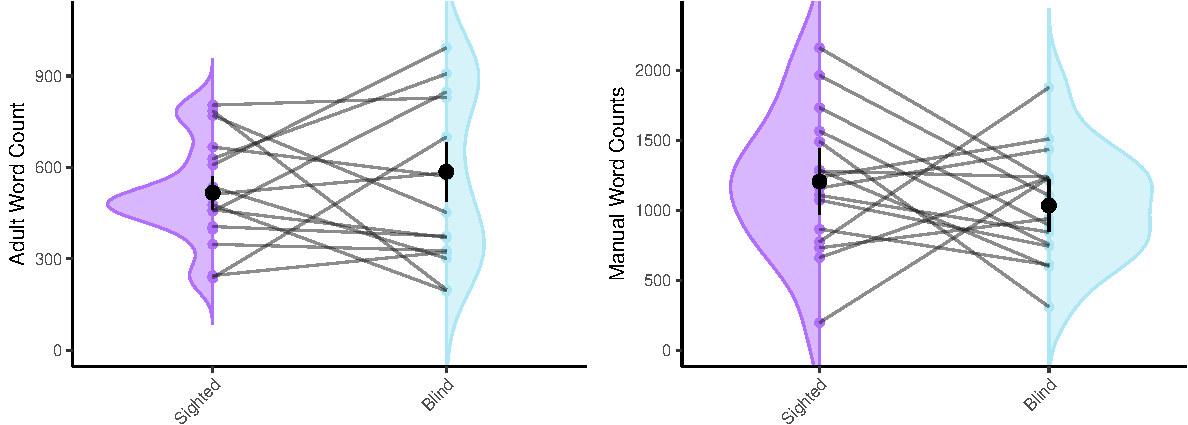
\includegraphics{input_quality_manuscript_files/figure-latex/quantity-plots-1.pdf}
\caption{\label{fig:quantity-plots}Comparing LENA-generated adult word counts (left) and transcription-based word counts in the input of blind and sighted children. Each dot represents the estimated number of words in one child's recording.}
\end{figure}

\hypertarget{language-input-quality}{%
\subsubsection{Language Input Quality}\label{language-input-quality}}

\hypertarget{interactiveness}{%
\paragraph{Interactiveness}\label{interactiveness}}

We compared the proportions of child-directed speech (CDS) between the blind children and their sighted matches. Each proportion was calculated as the number of utterances produced by someone \emph{other} than the target child (non-CHI utterances) tagged with a child or an adult addressee, respectively, out of the total number of non-CHI utterances for each sensory group. A two-sample test for equality of proportions revealed no significant difference in the overall proportions of CDS to blind children and CDS to sighted children.

We next compare the number of conversational turn counts for blind and sighted children, using LENA's automated Conversational Turn Count measure. A Wilcoxon rank-sum test shows that despite wide variability in the number conversational turns (210--1436 words\textsubscript{blind}, 112--1348 words\textsubscript{sighted}), blind and sighted children do not differ in the number of conversational turns (W = 120, \emph{p} = .794).

\begin{figure}
\centering
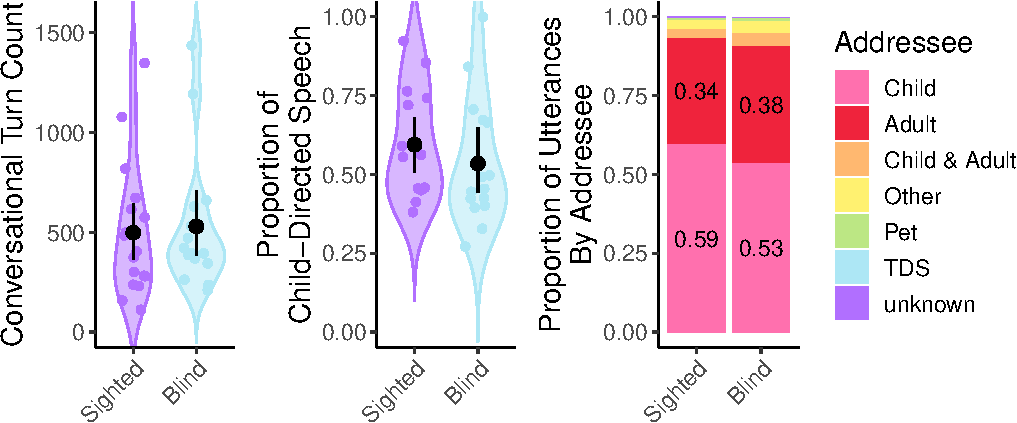
\includegraphics{input_quality_manuscript_files/figure-latex/interactiveness-plots-1.pdf}
\caption{\label{fig:interactiveness-plots}Comparing LENA-generated conversational turn counts (left) and proportion of utterances in child-directed speech (center). Each dot represents one child's recording. The full breakdown by addressee is shown in the rightmost panel.}
\end{figure}

\hypertarget{linguistic-features}{%
\paragraph{Linguistic Features}\label{linguistic-features}}

\begin{verbatim}
## 
##  Shapiro-Wilk normality test
## 
## data:  manual_word_TTR$TTR
## W = 0.95771, p-value = 0.2883
\end{verbatim}

\begin{verbatim}
## 
##  Welch Two Sample t-test
## 
## data:  manual_word_TTR$TTR by manual_word_TTR$group
## t = -1.2906, df = 26.749, p-value = 0.2079
## alternative hypothesis: true difference in means is not equal to 0
## 95 percent confidence interval:
##  -0.06732386  0.01534716
## sample estimates:
## mean in group TD mean in group VI 
##        0.3231817        0.3491700
\end{verbatim}

\begin{verbatim}
## 
##  Shapiro-Wilk normality test
## 
## data:  MLUs$MLU
## W = 0.91984, p-value = 0.0302
\end{verbatim}

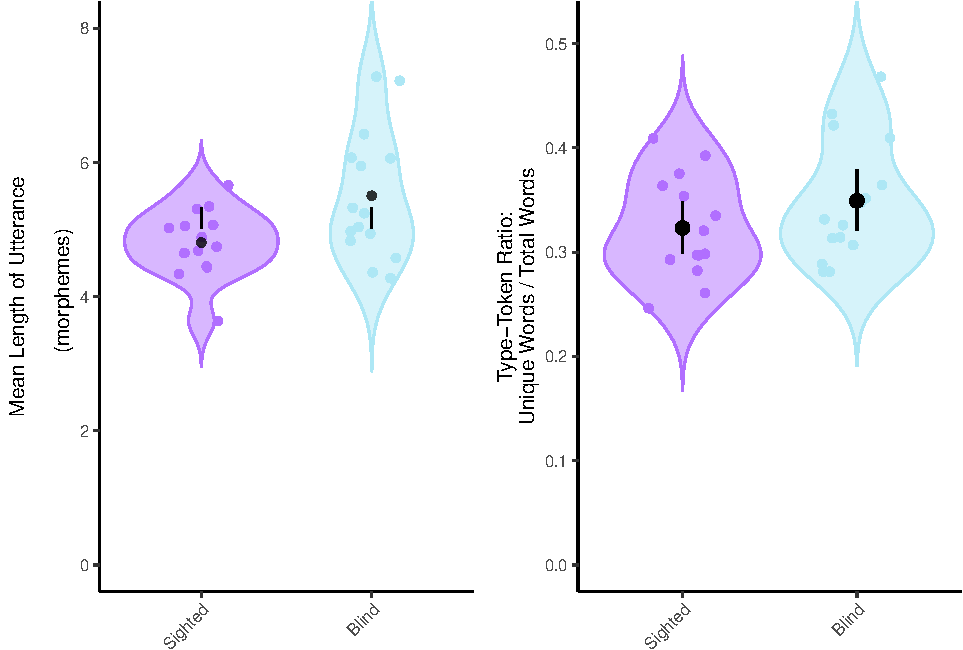
\includegraphics{input_quality_manuscript_files/figure-latex/linguistic-plots-1.pdf}

For linguistic features, we first measure proportion of unique words divided by the number of total words in the input, or type-token ratio, from the manual annotations. In order to compare the type-token ratio between blind and sighted children, we performed a Wilcoxon signed-rank test. The results of the Wilcoxon test indicated that there was no significant difference in the type-token ratio between the two groups (W = -1.29, p = .208). This suggests that, on average, the type-token ratio is similar for blind (M: 0.35) and sighted (M: 0.32) children (see Figure \ref{fig:TTR}). These results provide evidence that the variety of words in the input is not affected by children's vision.

\hypertarget{mlu-analysis-and-results}{%
\subparagraph{MLU Analysis and results}\label{mlu-analysis-and-results}}

For our second linguistic feature, we analyzed the mean length of utterance (MLU) in the input speech to each group of children. We computed MLU on a morpheme level as a proximate measure of syntactic complexity. Each utterance by a non-CHI speaker was tokenized into morphemes using the `morphemepiece' R package {[}CITE{]}. We then calculated the mean MLU per speaker from each audio recording, and then compared the mean MLU of environmental speech to blind children (M(SD) = XXX (XXX)) to that of sighted children (M(SD) = XXX (XXX)). A Wilcoxon rank-sum test revealed that the MLU was slightly but significantly higher in speech to blind children than to their sighted peers (W = , \emph{p} = .077).

\hypertarget{conceptual-features}{%
\paragraph{Conceptual Features}\label{conceptual-features}}

topic diversity - \url{https://github.com/mind-Lab/octis}
sensory modality
temporality

The last conceptual feature we examined is the displacement of events discussed in children's linguistic environment. That is, we tried to ascertain whether blind and sighted children receive a different amount of ``here-and-now'' commentary related to the events happening around them. Prior work has quantified such ``here-and-nowness'' by counting object presence co-occurring with a related noun label {[}CITE{]}. The audio format of our data and the coding scheme we use make it difficult to ascertain object presence, so instead of object displacement, in this analysis we will focus on temporal displacement. Notably, we are attempting to highlight semantic features of the language environment; however, given the constraints of large-scale textual analysis, we are categorizing utterances based on a combination of closely related syntactic and morphological features of verbs, since these contain time-relevant information. We recognize that these linguistic features do not perfectly align with the temporal structure of the world.

We assigned each utterance a \textbf{temporality} value: utterances tagged \emph{displaced} describe events that take place in the past, future, or irrealis space, while utterances tagged \emph{present} describe current, ongoing events. A small amount of utterances (n = 292) were left \emph{uncategorized} because they were fragments or because the automated parser failed to tag any of the relevant features. To do this, we used the udpipe package {[}CITE{]} to tag the transcriptions with parts of speech and other lexical features, such as tense, number agreement, or case inflection. To be marked as present, an utterance either had to be marked with both present tense and indicative mood, or appear in the gerund form with no marked tense (e.g.~\emph{you talking to Papa?}). Features that could mark an utterance as displaced included past tense, imperative mood, presence of a modal, presence of \emph{if}, or presence of \emph{gonna}/\emph{going to}, \emph{have to}, \emph{wanna}/\emph{want to}, or \emph{gotta}/\emph{got to}, since these typically indicate belief states and desires, rather than real-time events. In the case of utterances with multiple verbs, we selected the features from the first verb or auxiliary, as a proxy for hierarchical dominance.

The proportion of present versus displaced temporality did not differ between groups ().

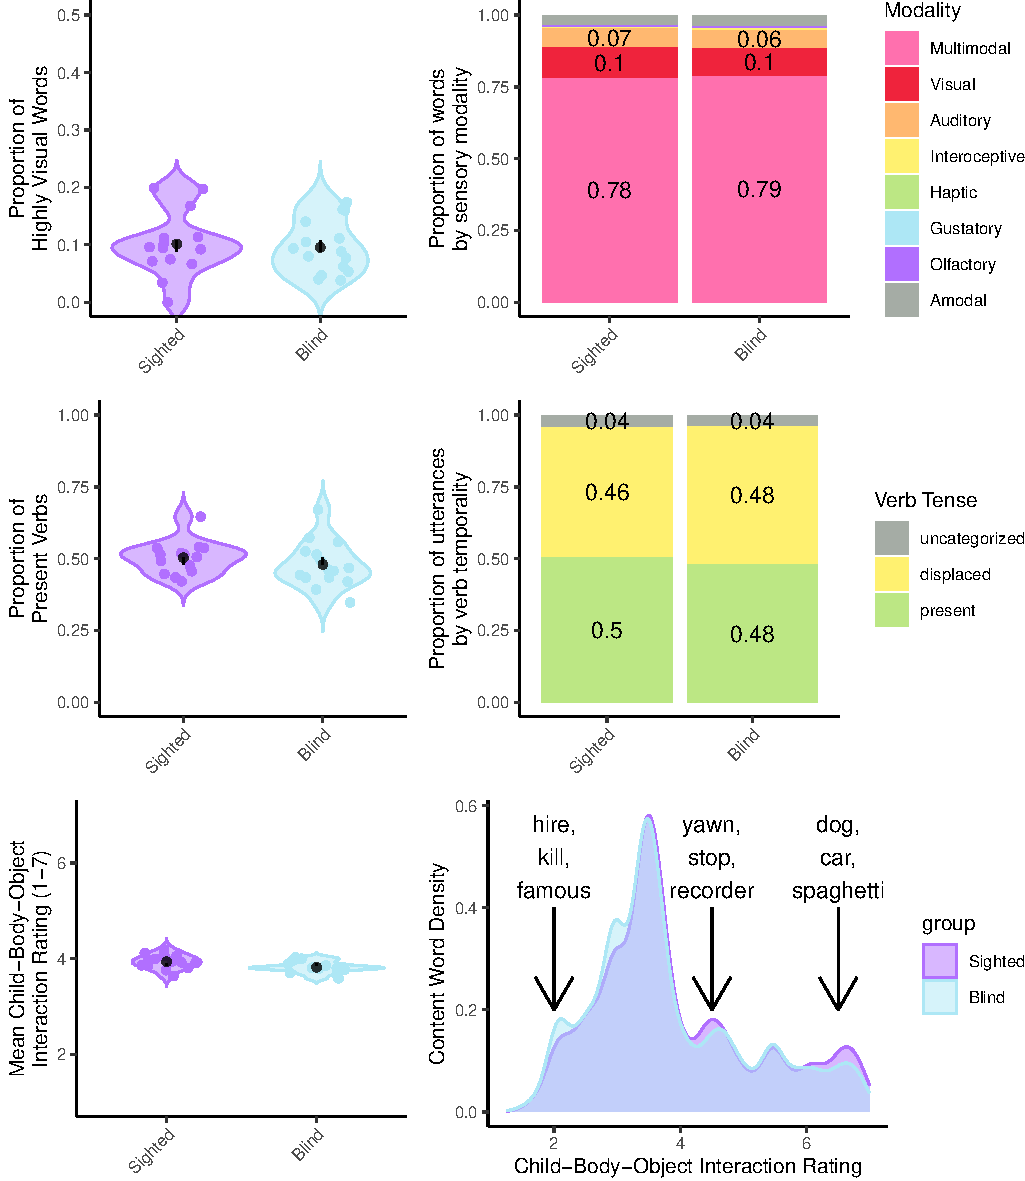
\includegraphics{input_quality_manuscript_files/figure-latex/conceptual-plots-1.pdf}

\hypertarget{linking-language-input-to-language-outcomes}{%
\subsection{Linking Language Input to Language Outcomes}\label{linking-language-input-to-language-outcomes}}

Predict: CDI percentile \& CVC percentile

\begin{verbatim}
## 
## Call:
## lm(formula = diff_age_from_expected ~ CDI_age_in_days + MLU + 
##     prop_present, data = lotta_data)
## 
## Residuals:
##      Min       1Q   Median       3Q      Max 
## -10.3779  -1.2762   0.6891   2.2429   5.4890 
## 
## Coefficients:
##                   Estimate Std. Error t value Pr(>|t|)    
## (Intercept)     -39.048910  11.140807  -3.505 0.002932 ** 
## CDI_age_in_days   0.018359   0.004551   4.034 0.000961 ***
## MLU               4.412389   1.375744   3.207 0.005493 ** 
## prop_present     22.350845  12.974226   1.723 0.104210    
## ---
## Signif. codes:  0 '***' 0.001 '**' 0.01 '*' 0.05 '.' 0.1 ' ' 1
## 
## Residual standard error: 4.153 on 16 degrees of freedom
##   (12 observations deleted due to missingness)
## Multiple R-squared:  0.6913, Adjusted R-squared:  0.6334 
## F-statistic: 11.94 on 3 and 16 DF,  p-value: 0.0002346
\end{verbatim}

\begin{figure}
\centering
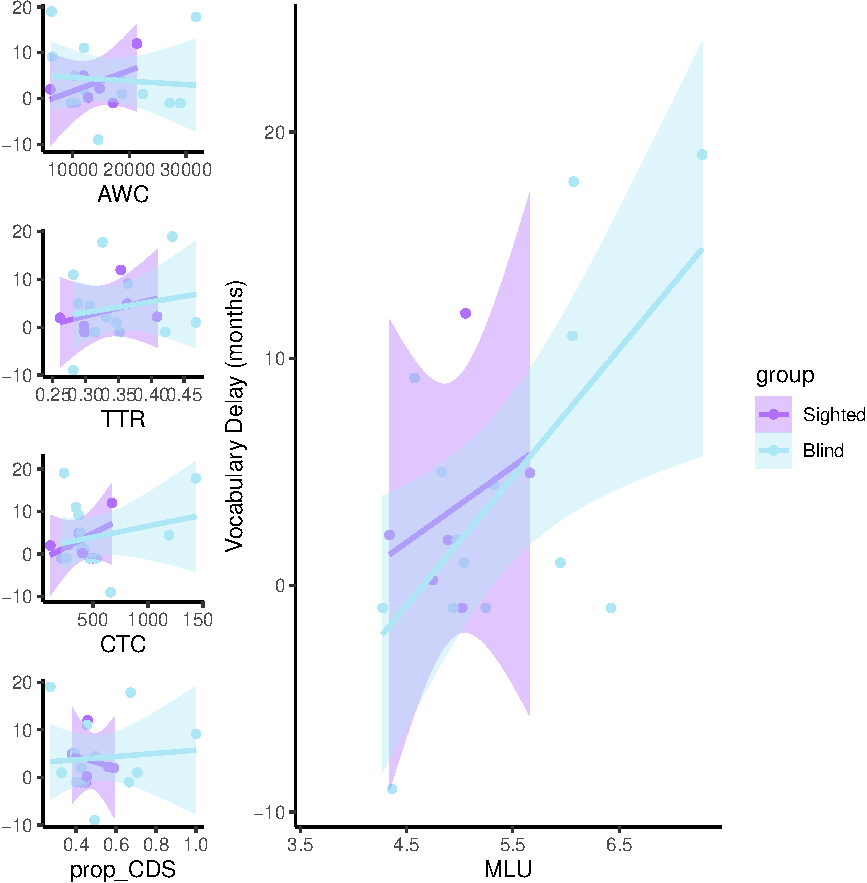
\includegraphics{input_quality_manuscript_files/figure-latex/predicting-plots-1.pdf}
\caption{\label{fig:predicting-plots}Plots of the relationship between the input variables and children's vocabulary outcomes (relative to the Wordbank 50th percentile.}
\end{figure}

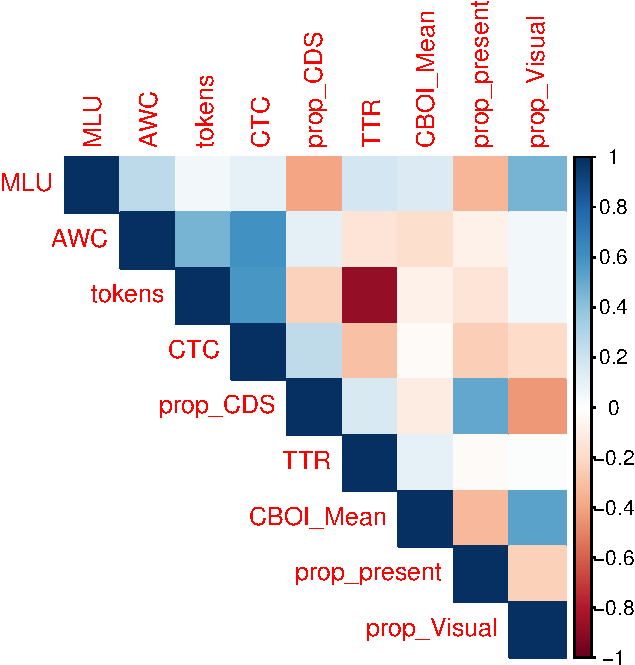
\includegraphics{input_quality_manuscript_files/figure-latex/variable-relationships-1.pdf} 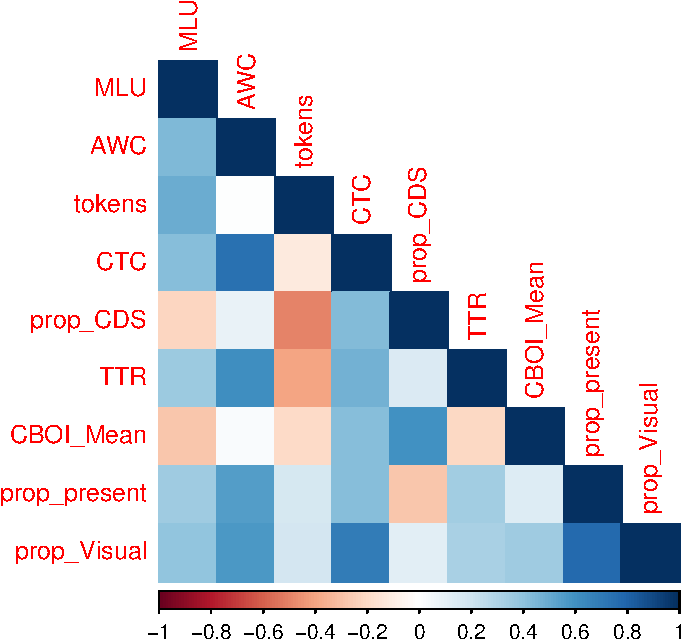
\includegraphics{input_quality_manuscript_files/figure-latex/variable-relationships-2.pdf}

\hypertarget{discussion}{%
\section{Discussion}\label{discussion}}

Sighted parents may be unfamiliar with blind children's signals of interest and engagement (Perez-Pereira \& Conti-Ramsden, 1999), and as a result, may respond less often to infants' vocalizations and bids for communication (Rowland, 1984). Might be hard to provide useful input due to differences in nonverbal communication between blind infants and their sighted caregivers. Young children born with visual impairment may differ in their nonverbal communication cues. For example, (G. M. Preisler, 1995) found that 6--9-month-old blind infants communicated using leaning, eyebrow raising, and lip movements. Caregivers who responded to these nonverbal cues as conversational turns had higher rates of interaction with the child, higher rates of appropriate response, and increased positive affect. By contrast, caregivers who did not recognize these signals as communicative had lower rates of response and increased negative affect.

\pagebreak

\hypertarget{references}{%
\section*{References}\label{references}}
\addcontentsline{toc}{section}{References}

\hypertarget{refs}{}
\begin{CSLReferences}{1}{0}
\leavevmode\vadjust pre{\hypertarget{ref-andersen1993}{}}%
Andersen, E. S., Dunlea, A., \& Kekelis, L. (1993). The impact of input: Language acquisition in the visually impaired. \emph{First Language}, \emph{13}(37), 23--49. \url{https://doi.org/10.1177/014272379301303703}

\leavevmode\vadjust pre{\hypertarget{ref-anderson2021}{}}%
Anderson, N. J., Graham, S. A., Prime, H., Jenkins, J. M., \& Madigan, S. (2021). Linking {Quality} and {Quantity} of {Parental Linguistic Input} to {Child Language Skills}: {A Meta-Analysis}. \emph{Child Development}, \emph{92}(2), 484--501. \url{https://doi.org/10.1111/cdev.13508}

\leavevmode\vadjust pre{\hypertarget{ref-bernsteinratner1984}{}}%
Bernstein Ratner, N. (1984). Patterns of vowel modification in mother\textendash child speech. \emph{Journal of Child Language}, \emph{11}, 557--578.

\leavevmode\vadjust pre{\hypertarget{ref-campbell2022}{}}%
Campbell, E. E., \& Bergelson, E. (2022). Making sense of sensory language: {Acquisition} of sensory knowledge by individuals with congenital sensory impairments. \emph{Neuropsychologia}, \emph{174}, 108320. \url{https://doi.org/10.1016/j.neuropsychologia.2022.108320}

\leavevmode\vadjust pre{\hypertarget{ref-campbell2003}{}}%
Campbell, J. (2003). Maternal {Directives} to {Young Children} who are {Blind}. \emph{Journal of Visual Impairment \& Blindness}, \emph{97}(6), 355--365. \url{https://doi.org/10.1177/0145482X0309700604}

\leavevmode\vadjust pre{\hypertarget{ref-chiesa2015}{}}%
Chiesa, S., Galati, D., \& Schmidt, S. (2015). Communicative interactions between visually impaired mothers and their sighted children: Analysis of gaze, facial expressions, voice and physical contacts. \emph{Child: Care, Health and Development}, \emph{41}(6), 1040--1046. \url{https://doi.org/10.1111/cch.12274}

\leavevmode\vadjust pre{\hypertarget{ref-devilliers1985}{}}%
De Villiers, J. (1985). Learning how to use verbs: Lexical coding and the influence of the input*. \emph{Journal of Child Language}, \emph{12}(3), 587--595. \url{https://doi.org/10.1017/S0305000900006668}

\leavevmode\vadjust pre{\hypertarget{ref-demir2015}{}}%
Demir, Ö. E., Rowe, M. L., Heller, G., Goldin-Meadow, S., \& Levine, S. C. (2015). Vocabulary, syntax, and narrative development in typically developing children and children with early unilateral brain injury: Early parental talk about the "there-and-then" matters. \emph{Developmental Psychology}, \emph{51}(2), 161--175. \url{https://doi.org/10.1037/a0038476}

\leavevmode\vadjust pre{\hypertarget{ref-donnellan2020}{}}%
Donnellan, E., Bannard, C., McGillion, M. L., Slocombe, K. E., \& Matthews, D. (2020). Infants' intentionally communicative vocalizations elicit responses from caregivers and are the best predictors of the transition to language: {A} longitudinal investigation of infants' vocalizations, gestures and word production. \emph{Developmental Science}, \emph{23}(1), e12843. \url{https://doi.org/10.1111/desc.12843}

\leavevmode\vadjust pre{\hypertarget{ref-fenson1994}{}}%
Fenson, L., Dale, P. S., Reznick, J. S., Bates, E., Thal, D. J., Pethick, S. J., \ldots{} Stiles, J. (1994). Variability in {Early Communicative Development}. \emph{Monographs of the Society for Research in Child Development}, \emph{59}(5), i. \url{https://doi.org/10.2307/1166093}

\leavevmode\vadjust pre{\hypertarget{ref-fernald1989}{}}%
Fernald, A. (1989). \href{https://www.ncbi.nlm.nih.gov/pubmed/2612255}{Intonation and communicative intent in mothers' speech to infants: Is the melody the message?} \emph{Child Development}, \emph{60}(6), 1497--1510.

\leavevmode\vadjust pre{\hypertarget{ref-ganea2018}{}}%
Ganea, N., Hudry, K., Vernetti, A., Tucker, L., Charman, T., Johnson, M. H., \& Senju, A. (2018). Development of adaptive communication skills in infants of blind parents. \emph{Developmental Psychology}, \emph{54}(12), 2265--2273. \url{https://doi.org/10.1037/dev0000564}

\leavevmode\vadjust pre{\hypertarget{ref-ganek2016}{}}%
Ganek, H., \& Eriks-Brophy, A. (2016). The {Language ENvironment Analysis} ({LENA}) system: {A} literature review. In \emph{Proceedings of the joint workshop on {NLP} for {Computer Assisted Language Learning} and {NLP} for {Language Acquisition}} (pp. 24--32). {Umeå, Sweden}: {LiU Electronic Press}.

\leavevmode\vadjust pre{\hypertarget{ref-gergle2004}{}}%
Gergle, D., Kraut, R. E., \& Fussell, S. R. (2004). Language {Efficiency} and {Visual Technology}: {Minimizing Collaborative Effort} with {Visual Information}. \emph{Journal of Language and Social Psychology}, \emph{23}(4), 491--517. \url{https://doi.org/10.1177/0261927X04269589}

\leavevmode\vadjust pre{\hypertarget{ref-gilkerson2018}{}}%
Gilkerson, J., Richards, J. A., Warren, S. F., Oller, D. K., Russo, R., \& Vohr, B. (2018). Language {Experience} in the {Second Year} of {Life} and {Language Outcomes} in {Late Childhood}. \emph{Pediatrics}, \emph{142}(4), e20174276. \url{https://doi.org/10.1542/peds.2017-4276}

\leavevmode\vadjust pre{\hypertarget{ref-goldstein2008}{}}%
Goldstein, M. H., \& Schwade, J. A. (2008). Social feedback to infants' babbling facilitates rapid phonological learning. \emph{Psychological Science}, \emph{19}(5), 515--523. \url{https://doi.org/10.1111/j.1467-9280.2008.02117.x}

\leavevmode\vadjust pre{\hypertarget{ref-grigoroglou2016}{}}%
Grigoroglou, M., Edu, U., \& Papafragou, A. (2016). Are children flexible speakers? {Effects} of typicality and listener needs in children's event descriptions. \emph{Cognitive Science}, 6.

\leavevmode\vadjust pre{\hypertarget{ref-hadley2017}{}}%
Hadley, P. A., Rispoli, M., Holt, J. K., Papastratakos, T., Hsu, N., Kubalanza, M., \& McKenna, M. M. (2017). Input {Subject Diversity Enhances Early Grammatical Growth}: {Evidence} from a {Parent-Implemented Intervention}. \emph{Language Learning and Development: The Official Journal of the Society for Language Development}, \emph{13}(1), 54--79. \url{https://doi.org/10.1080/15475441.2016.1193020}

\leavevmode\vadjust pre{\hypertarget{ref-hawkins2021}{}}%
Hawkins, R. D., Gweon, H., \& Goodman, N. D. (2021). The {Division} of {Labor} in {Communication}: {Speakers Help Listeners Account} for {Asymmetries} in {Visual Perspective}. \emph{Cognitive Science}, \emph{45}(3), e12926. \url{https://doi.org/10.1111/cogs.12926}

\leavevmode\vadjust pre{\hypertarget{ref-hirsh-pasek2015}{}}%
Hirsh-Pasek, K., Adamson, L. B., Bakeman, R., Owen, M. T., Golinkoff, R. M., Pace, A., \ldots{} Suma, K. (2015). The {Contribution} of {Early Communication Quality} to {Low-Income Children}'s {Language Success}. \emph{Psychological Science}, \emph{26}(7), 1071--1083. \url{https://doi.org/10.1177/0956797615581493}

\leavevmode\vadjust pre{\hypertarget{ref-hoff2003}{}}%
Hoff, E. (2003 Sep-Oct). The specificity of environmental influence: Socioeconomic status affects early vocabulary development via maternal speech. \emph{Child Development}, \emph{74}(5), 1368--1378. \url{https://doi.org/10.1111/1467-8624.00612}

\leavevmode\vadjust pre{\hypertarget{ref-hoff2002}{}}%
Hoff, E., \& Naigles, L. (2002 Mar-Apr). How children use input to acquire a lexicon. \emph{Child Development}, \emph{73}(2), 418--433. \url{https://doi.org/10.1111/1467-8624.00415}

\leavevmode\vadjust pre{\hypertarget{ref-hsu2017}{}}%
Hsu, N., Hadley, P. A., \& Rispoli, M. (2017). Diversity matters: Parent input predicts toddler verb production. \emph{Journal of Child Language}, \emph{44}(1), 63--86. \url{https://doi.org/10.1017/S0305000915000690}

\leavevmode\vadjust pre{\hypertarget{ref-huttenlocher1991}{}}%
Huttenlocher, J., Haight, W., Bryk, A., Seltzer, M., \& Lyons, T. (1991). Early vocabulary growth: {Relation} to language input and gender. \emph{Developmental Psychology}, \emph{27}, 236--248. \url{https://doi.org/10.1037/0012-1649.27.2.236}

\leavevmode\vadjust pre{\hypertarget{ref-huttenlocher2002}{}}%
Huttenlocher, J., Vasilyeva, M., Cymerman, E., \& Levine, S. (2002). Language input and child syntax. \emph{Cognitive Psychology}, \emph{45}(3), 337--374. \url{https://doi.org/10.1016/s0010-0285(02)00500-5}

\leavevmode\vadjust pre{\hypertarget{ref-huttenlocher2010}{}}%
Huttenlocher, J., Waterfall, H., Vasilyeva, M., Vevea, J., \& Hedges, L. V. (2010). Sources of variability in children's language growth. \emph{Cognitive Psychology}, \emph{61}(4), 343--365. \url{https://doi.org/10.1016/j.cogpsych.2010.08.002}

\leavevmode\vadjust pre{\hypertarget{ref-kekelis1984}{}}%
Kekelis, L. S., \& Andersen, E. S. (1984). Family {Communication Styles} and {Language Development}. \emph{Journal of Visual Impairment \& Blindness}, \emph{78}(2), 54--65. \url{https://doi.org/10.1177/0145482X8407800202}

\leavevmode\vadjust pre{\hypertarget{ref-landau1985}{}}%
Landau, B., \& Gleitman, L. R. (1985). \emph{Language and experience: {Evidence} from the blind child} (pp. xi, 250). {Cambridge, MA, US}: {Harvard University Press}.

\leavevmode\vadjust pre{\hypertarget{ref-macwhinney2019}{}}%
MacWhinney, B. (2019). {CHAT Manual}. \url{https://doi.org/10.21415/3MHN-0Z89}

\leavevmode\vadjust pre{\hypertarget{ref-naigles1998}{}}%
Naigles, L. R., \& Hoff-Ginsberg, E. (1998). Why are some verbs learned before other verbs? {Effects} of input frequency and structure on children's early verb use. \emph{Journal of Child Language}, \emph{25}(1), 95--120. \url{https://doi.org/10.1017/S0305000997003358}

\leavevmode\vadjust pre{\hypertarget{ref-newman2016}{}}%
Newman, R. S., Rowe, M. L., \& Bernstein Ratner, N. (2016). Input and uptake at 7 months predicts toddler vocabulary: The role of child-directed speech and infant processing skills in language development. \emph{Journal of Child Language}, \emph{43}(5), 1158--1173. \url{https://doi.org/10.1017/S0305000915000446}

\leavevmode\vadjust pre{\hypertarget{ref-ostarek2019}{}}%
Ostarek, M., Paridon, J. van, \& Montero-Melis, G. (2019). Sighted people's language is not helpful for blind individuals' acquisition of typical animal colors. \emph{Proceedings of the National Academy of Sciences}, \emph{116}(44), 21972--21973. \url{https://doi.org/10.1073/pnas.1912302116}

\leavevmode\vadjust pre{\hypertarget{ref-perez-pereira1999}{}}%
Perez-Pereira, M., \& Conti-Ramsden, G. (1999). \emph{Language {Development} and {Social Interaction} in {Blind Children}}. {London}: {Psychology Press}. \url{https://doi.org/10.4324/9780203776087}

\leavevmode\vadjust pre{\hypertarget{ref-preisler1991}{}}%
Preisler, Gunilla M. (1991). Early patterns of interaction between blind infants and their sighted mothers. \emph{Child: Care, Health and Development}, \emph{17}(2), 65--90. \url{https://doi.org/10.1111/j.1365-2214.1991.tb00680.x}

\leavevmode\vadjust pre{\hypertarget{ref-preisler1995}{}}%
Preisler, G. M. (1995). The development of communication in blind and in deaf infants--similarities and differences. \emph{Child: Care, Health and Development}, \emph{21}(2), 79--110. \url{https://doi.org/10.1111/j.1365-2214.1995.tb00412.x}

\leavevmode\vadjust pre{\hypertarget{ref-romeo2018}{}}%
Romeo, R. R., Leonard, J. A., Robinson, S. T., West, M. R., Mackey, A. P., Rowe, M. L., \& Gabrieli, J. D. E. (2018). Beyond the 30-{Million-Word Gap}: {Children}'s {Conversational Exposure Is Associated With Language-Related Brain Function}. \emph{Psychological Science}, \emph{29}(5), 700--710. \url{https://doi.org/10.1177/0956797617742725}

\leavevmode\vadjust pre{\hypertarget{ref-roseberry2014}{}}%
Roseberry, S., Hirsh-Pasek, K., \& Golinkoff, R. M. (2014 May-Jun). Skype me! {Socially} contingent interactions help toddlers learn language. \emph{Child Development}, \emph{85}(3), 956--970. \url{https://doi.org/10.1111/cdev.12166}

\leavevmode\vadjust pre{\hypertarget{ref-rowe2008}{}}%
Rowe, M. L. (2008). Child-directed speech: Relation to socioeconomic status, knowledge of child development and child vocabulary skill*. \emph{Journal of Child Language}, \emph{35}(1), 185--205. \url{https://doi.org/10.1017/S0305000907008343}

\leavevmode\vadjust pre{\hypertarget{ref-rowe2012}{}}%
Rowe, M. L. (2012). A {Longitudinal Investigation} of the {Role} of {Quantity} and {Quality} of {Child-Directed Speech} in {Vocabulary Development}. \emph{Child Development}, \emph{83}(5), 1762--1774. \url{https://doi.org/10.1111/j.1467-8624.2012.01805.x}

\leavevmode\vadjust pre{\hypertarget{ref-rowe2020}{}}%
Rowe, M. L., \& Snow, C. E. (2020). Analyzing input quality along three dimensions: Interactive, linguistic, and conceptual. \emph{Journal of Child Language}, \emph{47}(1), 5--21. \url{https://doi.org/10.1017/S0305000919000655}

\leavevmode\vadjust pre{\hypertarget{ref-rowland1984}{}}%
Rowland, C. (1984). Preverbal {Communication} of {Blind Infants} and {Their Mothers}. \emph{Journal of Visual Impairment \& Blindness}, \emph{78}(7), 297--302. \url{https://doi.org/10.1177/0145482X8407800701}

\leavevmode\vadjust pre{\hypertarget{ref-rubio-fernandez2019}{}}%
Rubio-Fernandez, P. (2019). Overinformative {Speakers Are Cooperative}: {Revisiting} the {Gricean Maxim} of {Quantity}. \emph{Cognitive Science}, \emph{43}(11), e12797. \url{https://doi.org/10.1111/cogs.12797}

\leavevmode\vadjust pre{\hypertarget{ref-senju2013}{}}%
Senju, A., Tucker, L., Pasco, G., Hudry, K., Elsabbagh, M., Charman, T., \& Johnson, M. H. (2013). The importance of the eyes: Communication skills in infants of blind parents. \emph{Proceedings. Biological Sciences}, \emph{280}(1760), 20130436. \url{https://doi.org/10.1098/rspb.2013.0436}

\leavevmode\vadjust pre{\hypertarget{ref-snow1972}{}}%
Snow, C. E. (1972). Mothers' {Speech} to {Children Learning Language} on {JSTOR}. \emph{Child Development}, \emph{43}, 549--565.

\leavevmode\vadjust pre{\hypertarget{ref-soderstrom2021}{}}%
Soderstrom, M., Casillas, M., Bergelson, E., Rosemberg, C., Alam, F., Warlaumont, A. S., \& Bunce, J. (2021). Developing a {Cross-Cultural Annotation System} and {MetaCorpus} for {Studying Infants}' {Real World Language Experience}. \emph{Collabra: Psychology}, \emph{7}(1), 23445. \url{https://doi.org/10.1525/collabra.23445}

\leavevmode\vadjust pre{\hypertarget{ref-tadic2013}{}}%
Tadić, V., Pring, L., \& Dale, N. (2013 Nov-Dec). Story discourse and use of mental state language between mothers and school-aged children with and without visual impairment. \emph{International Journal of Language \& Communication Disorders}, \emph{48}(6), 679--688. \url{https://doi.org/10.1111/1460-6984.12040}

\leavevmode\vadjust pre{\hypertarget{ref-thiessen2005}{}}%
Thiessen, E. D., Hill, E. A., \& Saffran, J. R. (2005). Infant-{Directed Speech Facilitates Word Segmentation}. \emph{Infancy: The Official Journal of the International Society on Infant Studies}, \emph{7}(1), 53--71. \url{https://doi.org/10.1207/s15327078in0701_5}

\leavevmode\vadjust pre{\hypertarget{ref-tomasello1986}{}}%
Tomasello, M., \& Farrar, M. J. (1986). Joint {Attention} and {Early Language}. \emph{Child Development}, \emph{57}(6), 1454. \url{https://doi.org/10.2307/1130423}

\leavevmode\vadjust pre{\hypertarget{ref-uccelli2019}{}}%
Uccelli, P., Demir-Lira, Ö. E., Rowe, M. L., Levine, S., \& Goldin-Meadow, S. (2019). Children's {Early Decontextualized Talk Predicts Academic Language Proficiency} in {Midadolescence}. \emph{Child Development}, \emph{90}(5), 1650--1663. \url{https://doi.org/10.1111/cdev.13034}

\leavevmode\vadjust pre{\hypertarget{ref-urwin1983}{}}%
Urwin, C. (1983). Dialogue and cognitive functioning in the early language development of three blind children: {Normal} and deficient, 142--161.

\leavevmode\vadjust pre{\hypertarget{ref-vygotsky1978}{}}%
Vygotsky, L. S., \& Cole, M. (1978). \emph{Mind in {Society}: {Development} of {Higher Psychological Processes}}. {Harvard University Press}.

\leavevmode\vadjust pre{\hypertarget{ref-weizman2001}{}}%
Weizman, Z. O., \& Snow, C. E. (2001). Lexical input as related to children's vocabulary acquisition: Effects of sophisticated exposure and support for meaning. \emph{Developmental Psychology}, \emph{37}(2), 265--279. \url{https://doi.org/10.1037/0012-1649.37.2.265}

\leavevmode\vadjust pre{\hypertarget{ref-yoshinaga-itano2020}{}}%
Yoshinaga-Itano, C., Sedey, A. L., Mason, C. A., Wiggin, M., \& Chung, W. (2020). Early {Intervention}, {Parent Talk}, and {Pragmatic Language} in {Children With Hearing Loss}. \emph{Pediatrics}, \emph{146}(Supplement\_3), S270--S277. \url{https://doi.org/10.1542/peds.2020-0242F}

\leavevmode\vadjust pre{\hypertarget{ref-yu2012}{}}%
Yu, C., \& Smith, L. B. (2012). Embodied attention and word learning by toddlers. \emph{Cognition}, \emph{125}(2), 244--262. \url{https://doi.org/10.1016/j.cognition.2012.06.016}

\leavevmode\vadjust pre{\hypertarget{ref-yurovsky2016}{}}%
Yurovsky, D., Doyle, G., \& Frank, M. C. (2016). Linguistic input is tuned to children's developmental level. \emph{Cognitive Science}, 6.

\end{CSLReferences}


\end{document}
